\documentclass[a4paper, titlepage]{article}

\usepackage[ngerman]{babel}
\usepackage[T1]{fontenc}
\usepackage[utf8]{inputenc}
\usepackage{graphicx}
\usepackage{amsmath}


\title{Die Gravitationskonstante g
auf einer schiefen Bahn}
\author{Sascha Huber, Aaron Stampa, Joanne Gautschi, Damien Flury}
\date{1. Dezember 2019}
\begin{document}
    \maketitle
    \tableofcontents
    \newpage
    \section{Experiment}
    Wir haben unser Experiment eingerichtet, wie auf Abbildung
    \ref{incline} dargestellt. Dann haben wir sieben mal
    einen Ball herunterrollen lassen mit verschieden Höhen
    \emph{h}. Die Länge \emph{x} ist die Distanz, in welcher
    wir die Objekte messen. Der Winkel $\theta$ bezeichnet
    den Winkel der schiefen Ebene in Bogenmass.

    \subsection{Ball auf der schiefen Ebene}
    Zunächst haben wir einen Ball herunterrollen lassen.
    Sein Radius \emph{r} beträgt etwa 4 cm, seine Masse
    \emph{m} 242 g.
    
    Wir haben die Strecke \emph{s} in Abhängigkeit
    der Zeit \emph{t} gemessen, um die Beschleunigung
    \emph{a} zu bestimmen. Dazu haben wir folgende Formel
    angewandt:
    \begin{equation}
        s = \frac{1}{2} \cdot a \cdot t^2
    \end{equation}
    Woraus folgt:
    \begin{equation}
        a = \frac{2 \cdot s}{t^2}
    \end{equation}
        

    \begin{figure}
        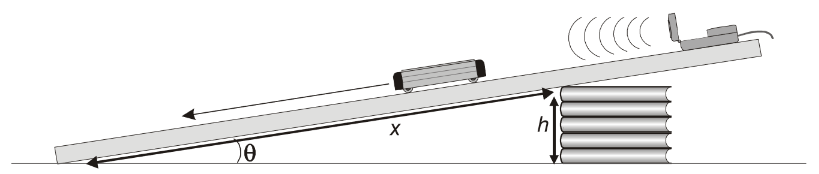
\includegraphics[width=\textwidth]{images/incline.png}
        \caption{Schiefe Bahn}
        \label{incline}
    \end{figure}


\end{document}